% MuJoCo 3.17 flex for the bonded PDMS skin: internals, verification against exact solutions, cell size, contact, robot.
% Build: latexmk -pdf flex_study.tex   (figures: python make_figs.py, reads ../compare, ../gt_transform, ../video)
\documentclass[10pt,twocolumn]{article}
\usepackage[letterpaper,margin=0.55in,top=0.55in,bottom=0.6in,columnsep=0.22in]{geometry}
\usepackage{mathptmx}
\usepackage[T1]{fontenc}
\usepackage{microtype,graphicx,booktabs,tikz,amsmath,enumitem,tabularx}
\usepackage[font=footnotesize,labelfont=bf,skip=3pt]{caption}
\usepackage[compact]{titlesec}
\usepackage[hidelinks]{hyperref}
\usetikzlibrary{patterns,decorations.pathmorphing,arrows.meta}
\titleformat*{\section}{\normalsize\bfseries}
\titleformat*{\subsection}{\small\bfseries\itshape}
\titlespacing*{\section}{0pt}{5pt}{2pt}
\titlespacing*{\subsection}{0pt}{3pt}{1pt}
\setlist{nosep,leftmargin=*}
\setlength{\parskip}{0pt}
\setlength{\textfloatsep}{6pt}
\setlength{\floatsep}{5pt}
\setlength{\abovedisplayskip}{3pt}\setlength{\belowdisplayskip}{3pt}
\setlength{\abovedisplayshortskip}{2pt}\setlength{\belowdisplayshortskip}{2pt}
\setlength{\emergencystretch}{1.5em}
\newcommand{\code}[1]{\texttt{\small #1}}
\newcommand{\src}[1]{\texttt{\footnotesize #1}}
\newcommand{\Nu}{N/\textmu m}
\newcommand{\um}{\,\textmu m}

\title{\vspace{-4mm}\large\textbf{MuJoCo 3.17 ``flex'' for our bonded PDMS skin: how it computes, how it compares with
exact solutions,\\ which cell size to use, and how to run it on the robot}\vspace{-2mm}}
\author{\small Dohyun, Jihoon \quad (AM/ME/CE 295, Caltech) \quad --- simulation study, 31 October 2026}
\date{\vspace{-7mm}}

\begin{document}
\maketitle

\noindent\textbf{Setting.} Each blade of the 2F-140 carries a PDMS layer $51\times71\times1.5$\,mm ($x$ across, $y$
along the finger, $z$ through), bonded at its back face, free at the front, read out by $5\times7$ taxels
($10.2\times10.14$\,mm). Material: linear elastic, $E=1$\,MPa, $\nu=0.45$ (placeholder; also 0.49 and, for the
ground truth, 0.499), $\rho=965$\,kg/m$^3$, no damping of any kind. Stiffnesses are in \Nu. Benchmarks:
P0 patch tests; G1 laterally confined layer; C1/C1f rigid platen over the whole face, no-slip/frictionless; C2
same, shear along $y$; C3 platen over $y\ge5.07$\,mm; C4 flat circular punch $a=5$\,mm; C5 sphere $R=10$\,mm to
30\um; C6/C6f square punch exactly over the centre taxel.

\noindent\textbf{Bottom line.} (i) MuJoCo's tetrahedral flex (\code{dof="full"}) uses a Lam\'e $\lambda$ twice too
large; a two-line input remap fixes it exactly. (ii) With the remap the elastic operator converges to the exact
solution from above at first order in the cell size: $+2.6$\,\% on a whole-face load and $+36$\,\% on a single-taxel
punch at 1.3\,mm cells. (iii) Contact is a penalty spring in series with the layer whose stiffness (in N/m) is
proportional to the vertex mass, so thinner elements make it softer; on the robot it is the dominant error. (iv) The
divergence on the robot is a separate MuJoCo defect (the per-island solver omits the flex stiffness);
\code{<flag island="disable"/>} cures it. (v) Contact is defined by where surfaces touch, not per taxel; in the exact
solution the neighbours of a pressed taxel bulge \emph{outward} slightly.

%==============================================================================
\section{What a flex is and how MuJoCo 3.17 computes it}
\label{sec:internals}
All code pointers are to the 3.17.0 tag (\src{src/}); they were re-checked for this report.

\textbf{Data model.} \code{<flexcomp type="grid" dim="3" count="11 15 3">} creates a vertex grid and splits every
hex into 6 tetrahedra with the \emph{same} body diagonal in every hex (\src{user/user\_mesh.cc:2703--2738}). With
\code{dof="full"} each unpinned vertex becomes a body with three slide joints (\src{user/user\_flexcomp.cc:529--540});
a pinned vertex (\code{<pin gridrange>}, our back face) is welded to the parent body (286--379). Every free vertex
gets \code{mass}/(number of points) and pinned vertices' share is dropped (476--477), so our flex carries 2/3 of the
specified mass. With \code{dof="trilinear"/"quadratic"} the degrees of freedom live on a coarse node grid
(\code{cellcount}) and the collision vertices follow by interpolation (580--706) \cite{mjdoc}.
Vertex joints inherit the parent's \code{childclass} armature, stiffness and frictionloss (all 0 in our model; keep
it so).


\begin{figure}[t]\centering
\resizebox{\columnwidth}{!}{%
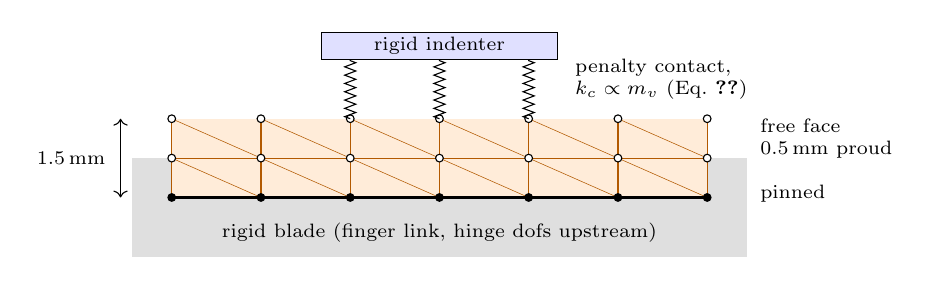
\begin{tikzpicture}[x=1.0cm,y=1.0cm,font=\scriptsize]
  % blade with pocket
  \fill[gray!25] (-0.2,-0.75) rectangle (7.6,0.0);
  \fill[gray!25] (-0.2,0.0) rectangle (0.3,0.5);
  \fill[gray!25] (7.1,0.0) rectangle (7.6,0.5);
  \node at (3.7,-0.45) {rigid blade (finger link, hinge dofs upstream)};
  % pdms
  \fill[orange!15] (0.3,0.0) rectangle (7.1,1.0);
  \foreach \x in {0.3,1.433,2.567,3.7,4.833,5.967,7.1} {\draw[orange!70!black,thin] (\x,0)--(\x,1.0);}
  \draw[orange!70!black,thin] (0.3,0.5)--(7.1,0.5);
  \foreach \x in {0.3,1.433,2.567,3.7,4.833,5.967} {\draw[orange!70!black,very thin] (\x,0.5)--(\x+1.133,0); \draw[orange!70!black,very thin] (\x,1.0)--(\x+1.133,0.5);}
  \draw[thick] (0.3,0)--(7.1,0);
  \foreach \x in {0.3,1.433,2.567,3.7,4.833,5.967,7.1} {\fill[black] (\x,0) circle (1.6pt); \draw[fill=white] (\x,0.5) circle (1.4pt); \draw[fill=white] (\x,1.0) circle (1.4pt);}
  % indenter + spring
  \fill[blue!12] (2.2,1.75) rectangle (5.2,2.1); \draw (2.2,1.75) rectangle (5.2,2.1);
  \node at (3.7,1.93) {rigid indenter};
  \draw[decorate,decoration={zigzag,segment length=3pt,amplitude=2pt}] (3.7,1.0)--(3.7,1.75);
  \draw[decorate,decoration={zigzag,segment length=3pt,amplitude=2pt}] (2.567,1.0)--(2.567,1.75);
  \draw[decorate,decoration={zigzag,segment length=3pt,amplitude=2pt}] (4.833,1.0)--(4.833,1.75);
  \node[anchor=west,align=left] at (5.3,1.5) {penalty contact,\\ $k_c\propto m_v$ (Eq.~\ref{eq:kc})};
  \node[anchor=east] at (-0.42,0.5) {1.5\,mm};
  \node[anchor=west,align=left] at (7.65,0.75) {free face\\0.5\,mm proud};
  \node[anchor=west] at (7.65,0.05) {pinned};
  \draw[<->] (-0.35,0)--(-0.35,1.0);
\end{tikzpicture}}
\caption{Cross-section of the model. Filled dots: back-face vertices pinned to the blade body; open dots: vertex
bodies with 3 slide joints each. Every hex is split into 6 tets along one fixed diagonal. Contact acts as a
mass-scaled penalty spring between the indenter and the layer.}
\label{fig:schematic}
\end{figure}

\textbf{Elasticity, \code{dof="full"} (Saint Venant--Kirchhoff on edges).} For a tet of rest volume $V$ with edge
lengths $l_e$ (rest $L_e$), $s_e=l_e^2-L_e^2$ and the Green strain is $E=\tfrac12\sum_e s_eB_e$, where $B_e$ is built
from the two face normals opposite edge $e$ (\code{ComputeBasis}, 1278--1310). At compile time
\code{ComputeStiffness} (1313--1342) and \code{MetricTensor} (1179--1220) form
\begin{equation}
k_{ef}= \mu V\,\mathrm{tr}(B_eB_f) + \lambda V\,\mathrm{tr}B_e\,\mathrm{tr}B_f ,
\end{equation}
and the energy evaluated at run time is $s^{\top}ks/4$ (comment at \src{engine\_core\_util.h:323}; forces:
\src{engine\_passive.c:587--640}). Substituting $E$:
\begin{equation}
W = V\big[\mu\,\mathrm{tr}E^2 + \lambda(\mathrm{tr}E)^2\big]\quad\text{vs.}\quad
W_{\rm StVK}=V\big[\mu\,\mathrm{tr}E^2 + \tfrac{\lambda}{2}(\mathrm{tr}E)^2\big],
\label{eq:W}
\end{equation}
i.e.\ $\lambda$ is doubled (finding F1, Sec.~\ref{sec:patch}). The energy depends only on edge lengths, so a mirrored
(inverted) tet stores no energy: there is no inversion barrier. The experimental Stable Neo-Hookean option
(\code{mjsFlex.elastic3d=1}, MjSpec only, changelog 3.15.0 item 5 \cite{mjchg}; \code{ComputeSNH} 1345--1372) has the
correct small-strain limit.

\textbf{Elasticity, interpolated (\code{trilinear}/\code{quadratic}).} Standard Galerkin linear elasticity,
$K=\int(\lambda\,\nabla\!\cdot u\,\nabla\!\cdot v+2\mu\,\varepsilon(u)\!:\!\varepsilon(v))$, fully integrated
(\code{ComputeLinearStiffness}, 1683--1768), co-rotational. Exact in the patch tests. (The \code{dim=2} membrane
path is 4$\times$ too soft in shear relative to its documented thickness; not used here.)

\textbf{Contact.} A \emph{plane} geom collides with each flex vertex (\src{engine\_collision\_flex.c:216--249}). Any
other geom (box, sphere, capsule, mesh) gets one GJK contact per surface-layer tet (\code{mjc\_ConvexElem}, 388):
the contact point is a tet corner that jumps between corners from step to step (median 7.2\,mm for a flat platen), and
its force is spread over the four corners by inverse distance (\src{engine\_core\_util.c:618--657, 785--830}), so
on average 21\,\% lands on vertices below the free face (up to 45\,\%). Contacts are soft constraints: for a contact on
one vertex of mass $m_v$ the regulariser is $R=\frac{1-d}{d}\,\mathrm{diag}A$ with $\mathrm{diag}A=1/m_v$. The resulting static
spring per vertex contact (measured to $10^{-6}$) is
\begin{equation}
k_c=\frac{d^2}{1-d}\,\frac{m_v}{d_{\max}^2\,\tau^2\zeta^2}\;\le\;\frac{0.9999}{0.0001}\,\frac{m_v}{h^2},
\label{eq:kc}
\end{equation}
($\tau,\zeta$ from \code{solref}, $d$ from \code{solimp}; the ceiling is the discrete-integrator floor on $R$,
\src{engine\_core\_constraint.c:2119--2121}). With the robot's \code{solref="1e-4 1"}, $d=0.99$ and
$m_v=10.6$\,mg (11$\times$15$\times$3 grid) $k_c=1.06\times10^5$\,N/m per vertex, 17.5\,\Nu{} over the free face:
only twice the layer's own 8.57\,\Nu. The ceiling is 69.6\,\Nu{} for the face at any \code{solref}. Contacts of
rigid and interpolated flexes are reduced to 50 per geom (\code{flexReducible},
\src{engine\_collision\_driver.c:572--575}; changelog 3.16.0 item 10).

\textbf{Discrete integrator.} Flex elasticity requires \code{integrator="discrete"} (implicit/implicitfast refuse it).
Each step solves for the velocity in the metric $\hat M=M+hD+h^2K$ by PCG (\code{mj\_effSolve},
\src{engine\_metric.c:1638--1714}) with 3$\times$3 vertex-block preconditioning when the flex is fixed to a static
body, and matrix-free with a mass preconditioner when its parent has joints. The PCG budget is
\code{opt.iterations}; exhausting it raises the ``too ill-conditioned'' warning, and a non-positive curvature exits
silently (1679--1681). A flex on a jointed parent (supported since 3.15 \cite{pr3618}) requires \code{solver="CG"} (\src{engine\_forward.c:1753}). Our layer
has $h\omega_{\max}=22$--916 at $h=0.5$\,ms and first thickness modes at 10.45\,kHz (compression) and 3.15\,kHz (shear),
$\omega h=32.8$ and 9.9; the integrator is accurate only for $\omega h\le0.3$ \cite{roqsim}. The elastic part is
unconditionally stable, but the layer's dynamics are numerically over-damped: \emph{treat the flex as quasi-static.}

%==============================================================================
\section{Verification against exact solutions}
\label{sec:verify}
\subsection{Ground truths (no MuJoCo involved)}
\textbf{Closed forms.} P0: $\sigma_{zz}=M\varepsilon$, $\tau=\mu\gamma$, $p=3K\varepsilon$. G1:
$K=MA/t$, $M=\lambda+2\mu$, which is also a rigorous \emph{upper} bound for C1 for any conforming discretisation.
\textbf{Infinite bonded layer} (\code{gt\_transform}): Fourier/Hankel transform of the Navier equations solved with
Papkovich--Neuber potentials, $u=0$ at $z=t$; checked symbolically, against an independent Chebyshev ODE solve
($\le2.7\times10^{-6}$), against both limits ($t/M$, half-space), and against the published kernel of
\cite{argatov}. Contact problems (C4, C5, C6) solved as integral equations (boundary elements, Richardson extrapolation) (C6 error
$\le9\times10^{-5}$). \textbf{Finite pad} (\code{gt\_fem}): 27-node quadratic bricks, graded to 0.1\,mm at edges,
three nested levels (up to 3.4\,M dof), mixed Q2/P1 form at $\nu=0.499$; verified by patch tests ($6\times10^{-13}$),
G1 ($10^{-14}$), manufactured solutions (rates 3.17/2.06 vs.\ 3/2) and a no-locking test of the mixed form. The two
ground truths agree within their error bars where they overlap (C4 to $2.7\times10^{-5}$, C6 to $1.2\times10^{-3}$).
C1--C3 are taken from the FEM, C4--C6 from the transform solution (Table~\ref{tab:gt}). For comparison, the classical thin-layer pressure method \cite{kelly} gives C1 $=7.337$\,\Nu{} ($-14.3$\,\%) at $\nu=0.45$.

\begin{table}[t]\centering\footnotesize
\caption{Ground truth (\Nu; C5 force in N, contact radius $a$ in mm). Errors: C1--C3 $\le0.05$\,\%, C4--C6
$\le10^{-4}$. $GA/t=0.8324$ at $\nu=0.45$. $MA/t$ (Winkler line, comparison only) is $+6.9$, $+22$, $+108$\,\% above C1.}
\label{tab:gt}
\begin{tabular}{@{}lrrr@{}}\toprule
case & $\nu=0.45$ & 0.49 & 0.499\\\midrule
G1 $=MA/t$ & 9.1566 & 41.313 & 403.41\\
C1 platen, no-slip & 8.5662 & 33.757 & 194.33\\
C1f platen, frictionless & 8.0102 & 27.252 & 91.727\\
C2 platen shear along $y$ & 0.82791 & 0.80602 & 0.80126\\
C3 half platen & 3.5927 & 13.139 & 55.376\\
C4 punch $a=5$, frictionless & 0.14757 & 0.24139 & 0.28798\\
C6 taxel punch, no-slip & 0.21658 & 0.48158 & 0.73233\\
C6f taxel punch, frictionless & 0.19971 & 0.34327 & 0.42106\\
C5 $R=10$\,mm, $F$(30\um) [N] & 0.04397 & 0.04822 & 0.04938\\
C5 contact radius $a$ [mm] & 0.632 & 0.640 & 0.642\\\bottomrule
\end{tabular}
\end{table}

Two physical facts follow. Going from $\nu=0.45$ to the realistic 0.49--0.499 raises flat-contact stiffness 2--3.4$\times$
(shear is unchanged), so the placeholder matters. And the Winkler foundation ($k=M/t$) is not a usable reference:
$+35$\,\% on C4 at $\nu=0.45$, up to 30$\times$ at 0.499, and the wrong shape for the sphere.

\subsection{Patch tests and the doubled \texorpdfstring{$\lambda$}{lambda} (F1)}
\label{sec:patch}
Exact homogeneous strains were imposed and \code{qfrc\_spring} compared with the exact nodal forces
(Table~\ref{tab:patch}). Fitting $f=\mu f_\mu+\lambda f_\lambda$ gives $\lambda_{\rm eff}/\lambda=2.00000$ (residual
$<10^{-11}$) and $\mu_{\rm eff}/\mu=1.00000$ for $\nu=0.3$, 0.45, 0.49, on a cube and on our layer, with rotated and
moving parents, and at 1\,\% finite strain: Eq.~\eqref{eq:W} exactly. The simulated material at $\nu=0.45$ is
$\nu_{\rm eff}=0.4737$ with $E$ almost unchanged ($\times1.016$) but bulk modulus $\times1.931$ and confined modulus
$\times1.818$. This is why nobody noticed: MuJoCo's own test uses $\nu=0$
(\src{test/engine/engine\_passive\_test.cc:578}) \cite{mjtest}, and the validations we found are cantilevers or
unconfined blocks; a thin bonded layer is the worst case. No upstream report exists (searched in the survey;
PR \#3621 only notes that ``the previous 3D StVK volumetric normalization is preserved'' \cite{pr3621}).

\begin{table}[t]\centering\footnotesize
\caption{P0 patch tests: energy ratio MuJoCo/exact over 154 models (from \code{bench\_static}).}
\setlength{\tabcolsep}{3.5pt}
\label{tab:patch}
\begin{tabular}{@{}lccc@{}}\toprule
variant & uniaxial strain & simple shear & hydrostatic\\\midrule
full, raw inputs, $\nu=0.45$ & 1.818182 & 1.000000 & 1.931034\\
full, raw inputs, $\nu=0.49$ & 1.960784 & 1.000000 & 1.986577\\
full remapped; trilinear; quadratic & 1.000000 & 1.000000 & 1.000000\\\bottomrule
\end{tabular}
\end{table}

\textbf{Workaround} (exact, verified): pass
$\nu_{\rm in}=\nu/(2(1-\nu))$, $E_{\rm in}=E(1+\nu_{\rm in})/(1+\nu)$, which keeps $\mu$ and feeds $\lambda/2$:
$\nu=0.45\Rightarrow$ \code{young="971787" poisson="0.409091"}; $\nu=0.49\Rightarrow$ \code{993552}, \code{0.480392}.
\textbf{Upstream fix:} in \code{ComputeStiffness} (\src{user\_flexcomp.cc:1325}) divide \code{la} by 8 instead of 4
(not in \code{MetricTensor}, which the SNH path reuses with \code{la}$=-\mu$). A report draft with a 17-line repro
(one tet; prints ratios 1.8182 and 2.0000) is in \code{study/internals/bug\_lambda.md}; it has not been posted.

\subsection{The elastic operator vs.\ ground truth}
To separate discretisation from contact, MuJoCo's own stiffness was extracted by finite differences of
\code{qfrc\_spring} (symmetric to $7\times10^{-10}$, equal to MuJoCo's assembled matrix to $1.6\times10^{-9}$) and
loaded with exact displacement boundary conditions on 295 meshes. Table~\ref{tab:static} gives the errors. With F1
uncorrected the current robot grid is $+85$\,\% on C1; F1 is the dominant error for distributed loads. Corrected,
every element type converges from above, consistent with the $MA/t$ bound. Shear (C2) is within 0.55\,\% on every
mesh. At $\nu=0.499$ all linear elements lock (corrected full flex with 6 elements through the thickness is still
$+5.5$\,\% on C1). The single fixed tet diagonal also biases local loads: a normal load on the centre taxel produces a
spurious in-plane displacement of 16\,\% of $u_z$ on the 11$\times$15$\times$3 grid (6\,\% at 21$\times$29$\times$5),
which a mirrored split removes.

\begin{table}[t]\centering\footnotesize
\caption{Discretisation error of MuJoCo's elastic operator (exact BCs, no contact), $\nu=0.45$, \%. Meshes in
cells $n_x\times n_y\times n_z$ (vertices $=$ cells $+1$); the robot grid 11$\times$15$\times$3 vertices is
10$\times$14$\times$2 cells (5.1\,mm).}
\label{tab:static}
\setlength{\tabcolsep}{3.2pt}
\begin{tabular}{@{}lrrrrr@{}}\toprule
mesh & C1 & C1f & C2 & C3 & C6\\\midrule
10$\times$14$\times$2, raw (robot now) & $+85.3$ & $+77.3$ & $+0.5$ & $+100.4$ & $+345$\\
10$\times$14$\times$2, F1-corrected & $+4.4$ & $+4.8$ & $+0.5$ & $+14.2$ & $+158$\\
5$\times$7$\times$1, corrected & $+6.9$ & $+9.2$ & $+0.5$ & $+26.1$ & $+371$\\
40$\times$56$\times$2, corrected (1.275\,mm) & $+2.6$ & $+2.3$ & $+0.5$ & $+5.1$ & $+36.3$\\
quadratic 40$\times$56$\times$3 & $+0.3$ & $+0.3$ & $+0.2$ & $+0.7$ & $+5.1$\\\midrule
40$\times$56$\times$2 corrected, $\nu=0.49$ & $+7.8$ & & & $+14.1$ & $+110$\\\bottomrule
\end{tabular}
\end{table}

%==============================================================================
\section{Cell size: accuracy, cost, convergence}
\label{sec:cells}

\begin{figure*}[t]\centering
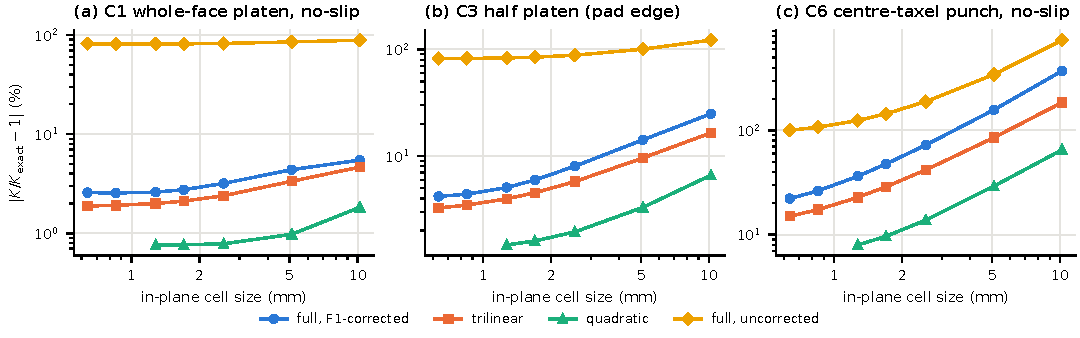
\includegraphics[width=\textwidth]{fig/conv.pdf}
\caption{Discretisation error vs.\ in-plane cell size (2 elements through the thickness; quadratic: 1 cell),
$\nu=0.45$. Fitting $e=a\,\Delta x^p+b\,\Delta z^q$ gives $p=0.76$, 0.97, 1.22 for C1, C3, C6 (full, corrected):
first order, as the edge singularities allow; quadratic elements lower the constant, not the order. The raw
(uncorrected) flex has an $\approx$80\,\% floor on distributed loads.}
\label{fig:conv}
\end{figure*}

\begin{figure*}[t]\centering
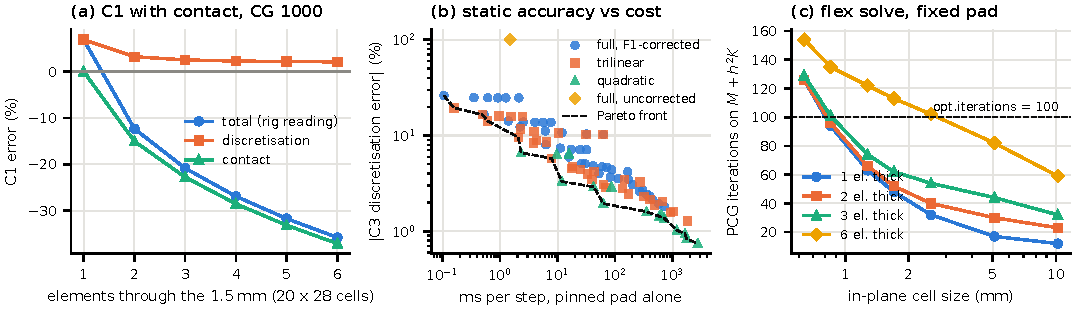
\includegraphics[width=\textwidth]{fig/cost.pdf}
\caption{(a) Whole-face platen with contact (robot contact setting, 20$\times$28 cells): the static error saturates,
but each extra element through the thickness makes the contact (and the total reading) softer.
(b) Static accuracy against time per step for all 295 meshes (shared machine; indicative). (c) PCG iterations of the
flex solve ($M+h^2K$, fixed pad) against in-plane cell size; above 100 the default budget is exceeded.}
\label{fig:cost}
\end{figure*}

\textbf{In-plane size} (Fig.~\ref{fig:conv}). Convergence is first order for every element type. For distributed
loads (C1, C3) refinement below $\approx$2.5\,mm buys little: with contact, C1 moves from $-12.4$ to $-13.7$\,\% between
2.55 and 1.275\,mm while cost rises 4.4$\times$ and the contact count 3.8$\times$. For localized loads the error
falls only as $\Delta x^{1.2}$: C6 is $+72$, $+36$, $+15$\,\% at 2.55, 1.275, 0.64\,mm. The C5 sphere's exact contact
radius (0.63\,mm) is smaller than any affordable uniform cell, so C5 is $+313$\,\% at 1.275\,mm.

\textbf{Through the thickness} (Fig.~\ref{fig:cost}a). The static error saturates after 2--3 elements (C1 $+3.2$,
$+2.5$, $+2.3$\,\% for 2, 3, 4 at 2.55\,mm). With contact, more elements make the reading \emph{worse}: by
Eq.~\eqref{eq:kc} the contact stiffness scales with the vertex mass, and thinner elements mean lighter surface vertices.
The contact error is $-15$, $-23$, $-29$, $-33$, $-37$\,\% for 2--6 elements; the total goes from $-12$ to $-36$\,\%.
Each added element also costs 1.3--1.4$\times$ and adds PCG iterations (40, 54, 70, 86, 102 at 2.55\,mm for 2--6).
This is the \textbf{overmeshing} to avoid: through-thickness refinement beyond 2 elements, and in-plane refinement
below 2.5\,mm for distributed loads.

\textbf{Solver convergence.} The stiffness of the discretised layer makes $\mathrm{cond}(M+h^2K)$ range from 34 to
$6.1\times10^4$, set mainly by the element thickness. The flex PCG needs 12--419 iterations and exceeds the default 100
at $\approx$0.85\,mm cells (Fig.~\ref{fig:cost}c). The contact solve is the harder part: with the robot's elliptic cone
and \code{impratio=100}, no-slip contact never converges in 100 CG iterations on any mesh (every step hits the cap;
force chatter $3\times10^{-2}$ to $2\times10^{-1}$, and the C2 shear force flips sign). With 1000 iterations the median
is 480--800 and the force settles within $\approx$1\,ms on 2.55\,mm or finer meshes. Frictionless contact converges in
15--70 iterations.

\textbf{Recommended cell structure.} \emph{Robot} (budget 1--5\,ms per step): 6$\times$8$\times$2 vertices
(5$\times$7$\times$1 cells), one element per taxel with grid lines on the taxel borders and one through the thickness,
F1-corrected. \emph{Fixed rig} (sensor studies): 41$\times$57$\times$3 vertices (40$\times$56$\times$2 cells,
$1.275\times1.268\times0.75$\,mm), and for an indenter at a known position a graded tet mesh
(\code{flexcomp type="direct"}): with a 0.5\,mm core C4, C6, C6f are $+14.8\pm7.3$, $+16.6\pm10.0$, $+17.8\pm7.8$\,\%,
and with a 0.15\,mm core C5 is $+11.6$\,\%, at 0.1--0.5\,s per step and with only 3--5\,\% of the indentation taken by
contact penetration. Table~\ref{tab:choice} gives the total errors (contact included) of both choices. Interpolated
flexes, though most accurate per dof statically, are rejected with contact: the 50-contact cap makes their apparent
stiffness collapse with refinement (trilinear C1f 1.82, 0.36, 0.10\,\Nu{} at 10$\times$14$\times$2, 20$\times$28$\times$3,
40$\times$56$\times$3) and no-slip shear fails ($-93$ to $-133$\,\%).

\begin{table}[t]\centering\footnotesize
\caption{Total error (\%, contact included, $\nu=0.45$) of the recommended structures on the rig; $\pm$ is the 95\,\%
interval over 5 indenter placements. Rig: \code{solref 1e-4}, CG 1000. Robot: \code{solref 1e-3}, CG 100.}
\label{tab:choice}
\setlength{\tabcolsep}{4pt}
\begin{tabular}{@{}lrrr@{}}\toprule
case & rig 40$\times$56$\times$2 & (discretis.\,/\,contact) & robot 5$\times$7$\times$1\\\midrule
C1 & $-13.7$ & $+2.6\,/\,{-15.9}$ & $-89.0$\\
C1f & $-12.6$ & $+2.3\,/\,{-14.6}$ & $-88.3$\\
C2 & $-8.2$ & $+0.5\,/\,{-8.7}$ & $-41.1$\\
C3 & $-12.4$ & $+5.1\,/\,{-16.7}$ & $-88.4$\\
C4 & $+8.4\pm7.0$ & $-1.8\,/\,{+10.4}$ & $-70.7\pm13.9$\\
C6 & $+9.1\pm24.8$ & $+36.3\,/\,{-20.0}$ & $-76.4\pm5.5$\\\bottomrule
\end{tabular}
\end{table}

On the rig, the good C4/C6 numbers of the uniform mesh are a \emph{cancellation} ($+36$\,\% discretisation, $-20$\,\%
contact) with a $\pm25$\,\% dependence on where the punch sits relative to the grid; the graded mesh's errors are
genuine. At $\nu=0.49$ the layer is 4$\times$ stiffer but the contact is not, so the contact error doubles (rig C1
$-46.9$\,\%). For deformation studies read the layer from the vertex positions (\code{flexvert\_xpos}), not from the
indenter travel.

%==============================================================================
\section{Contact with objects: what the layer does}
\label{sec:contact}

\begin{figure}[t]\centering
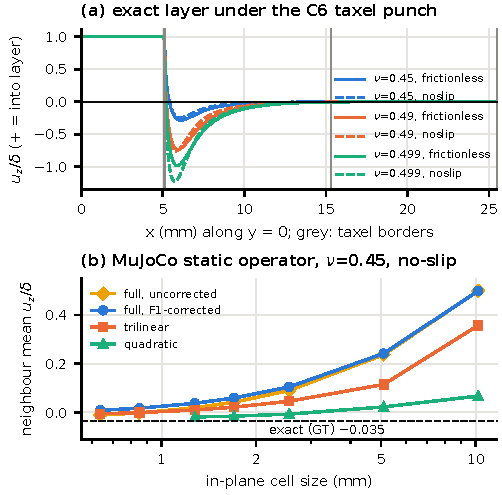
\includegraphics[width=\columnwidth]{fig/crosstalk.pdf}
\caption{(a) Exact surface displacement along $y=0$ under the C6 taxel punch (gt\_transform). Outside the punch the
surface rises; the neighbours carry no contact force. (b) Mean $u_z/\delta$ of the four neighbouring taxels in
MuJoCo's static operator vs.\ cell size; positive values on coarse meshes are interpolation spill-over through
shared nodes.}
\label{fig:crosstalk}
\end{figure}

\textbf{Is contact defined per cell?} No. In MuJoCo, as in the continuum, contact exists where the surfaces touch;
\code{tactile.py} (\code{PDMSSkin}) bins each contact force into the taxel that contains its contact point. In the exact
solution for the C6 punch the contact force is 100\,\% in the centre taxel and exactly zero in the neighbours, and the
neighbouring surfaces do not follow the punch: they bulge outward (Fig.~\ref{fig:crosstalk}a). The mean $u_z/\delta$
of the edge neighbours is $-0.047/-0.035$ (frictionless/no-slip) at $\nu=0.45$, $-0.147/-0.127$ at 0.49 and
$-0.200/-0.202$ at 0.499; the peak rise just outside the punch edge is 0.29, 0.74 and 0.99$\delta$. So \emph{if cells
1,\,2,\,3 deform $+1,+2,+1$, the outer cells must themselves be touched} (and carry force), or the pattern is a mesh
artefact: pressing cell 2 alone by 2 units moves cells 1 and 3 by about $-0.07$. What does spread is the force
transmitted to the rigid blade: at the bond plane the centre cell takes 84.2/88.5\,\% (0.45) and each edge neighbour
1.6--3.6\,\%.

MuJoCo's static operator reproduces this only on fine meshes (Fig.~\ref{fig:crosstalk}b): on the robot grid the
neighbours move $+0.22$ to $+0.25\delta$ (and unequally, 0.252 vs.\ 0.223, because of the fixed tet diagonal);
quadratic elements at 1.275\,mm give $-0.024$. With contact, the force still bins only into touched taxels; neighbours
get displacement only (27--35\,\% of the centre at 10$\times$14$\times$2, 0.3--7\,\% at 40$\times$56$\times$3).

\begin{figure*}[t]\centering
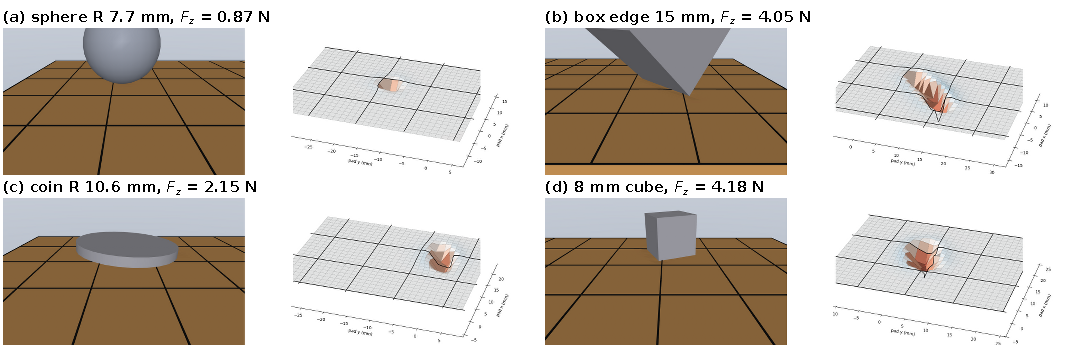
\includegraphics[width=0.84\textwidth]{fig/stills.pdf}
\caption{Frames from the close-up video at full normal load, before sliding (each pair: true-scale MuJoCo render with
taxel borders; free-face displacement exaggerated 40$\times$, colour $=u_z$ in \textmu m). 40$\times$56$\times$3 cells,
F1-corrected, \code{solref 3e-6}, \code{solimp 0.9999}, CG 3000. Video:
\code{docs/media/flex\_contact\_closeup.mp4} (1920$\times$1080, 41.7\,s, 8 objects: approach, press, hold,
slide 2.1--4.0\,mm, hold, lift-off).}
\label{fig:stills}
\end{figure*}

\textbf{Close-up video} (Fig.~\ref{fig:stills}). Eight rigid objects (sphere, rod, box edge, book corner, capsule,
ellipsoid, coin, cube) are pressed into the fixed pad by servo-driven slide joints, slid and lifted. All runs are free
of NaN and inverted tets (minimum volume ratio 0.754), CG never hits its cap, the taxel forces sum to the total contact
force to $5\times10^{-15}$\,N, and the residual displacement after lift-off is $\le1.2\times10^{-4}$\um. The displacement
is one continuous field across taxel borders while force goes only to touched taxels; for the cube: taxel (3,3)
3.18\,N with mean $u_z=14.1$\um, (3,4) 0.61\,N and 3.8\um, (3,2) 0\,N and $-0.1$\um. Limitations, stated plainly:
(i) a 1\,MPa, 1.5\,mm layer indented by tens of micrometres carries only $\approx$1\,N under a curved object; seven of
eight objects stopped at the 100\um{} indentation cap at 0.7--4.2\,N, not the 5--20\,N targets. A 250\um{} cap
inverted 6 surface tets during sliding, which stayed inverted after lift-off (no inversion barrier).
(ii) Even with the stiffest contact, penetration is 11--30\,\% of $u_z$. (iii) Contacts smaller than a cell are
under-resolved (the sphere dimple is 1--2 vertices wide; the book corner hops between vertices). (iv) With no material
damping, the hold rings (cube: 6.6\um{} std).

%==============================================================================
\section{Running it on the robot}
\label{sec:robot}
\textbf{Failure.} Pinned to the blade inside the 2F-140, the full flex diverged within $\approx$3 steps whenever any
upstream joint was free. \textbf{Cause} (found in the source, reproduced in a minimal model, fixed in an instrumented
build): the constraint solver works per \emph{island}, and the island metric operator selects flexes with
\code{flexMatrixFree} (\src{engine\_metric.c:2485--2491}), which gates on \code{mjd\_flexStiff\_active}
(\src{engine\_derivative.c:1901--1908}). That returns 0 for any flex that is not ``simple'', i.e.\ pinned to a body
with joints. The monolithic operator \code{mj\_effMulAdd} (\src{engine\_metric.c:236--246}) does include such flexes,
so the smooth acceleration is right but the constraint correction is computed with $M$ alone. The largest generalised
eigenvalue of $(M+S_{\rm isl})^{-1}(M+S_{\rm mono})$ is $1.5\times10^4$ on the robot (1.000 with the fix), equivalent
to explicit integration at $h\omega\approx120$. Any constraint row creates an island (mimic equalities, a joint limit,
a contact), which is why locking all joints was stable. The PCG budget is \emph{not} the cause (the home pose needs
116 iterations against 100, hence the warning; the solve never takes the $pAp\le0$ exit). Minimal repro: one hinge, a
pinned 3$\times$3$\times$2 flex and one joint equality diverge at step 3 (\code{study/robot/repro/minimal\_repro.xml}).
\textbf{Fix:} \code{<flag island="disable"/>}, or the one-function patch \code{study/robot/fix/island\_flex\_fix.patch}
(same results).

\textbf{Second problem: the contact setting.} With islands off, the robot's \code{solref="1e-4 1"} (time constant
$h/5$) and CG 100 overload the layer ($\approx$1000\,N per side within 25\,ms against a 120\,N squeeze); it turns
inside out (798/866 inverted tets, free face 1.6--3.0\,mm in) and the box ends up held by the rigid rims. Two settings
work (Table~\ref{tab:robot}): A keeps the stiff contact and lets CG converge; B softens the contact to $\tau=2h$.

\begin{table}[t]\centering\footnotesize
\caption{2.7\,s close-and-lift with both pads, islands off, F1-corrected; held force L/R, load on the rigid blade,
largest contact penetration, wall time per 0.5\,ms step (single thread, shared machine). A uses tolerance $10^{-10}$.}
\label{tab:robot}
\setlength{\tabcolsep}{3pt}
\begin{tabular}{@{}llrrrr@{}}\toprule
grid & \code{solref}\,/\,CG its & held L/R (N) & rim (N) & pen.\,(mm) & ms/step\\\midrule
11$\times$15$\times$3 & now: \code{1e-4}/100 & $45/28$ & 158 & 0.03 & 24.1\\
11$\times$15$\times$3 & A: \code{1e-4}/1000 & 120.2/120.1 & 0 & 0.055 & 145\\
11$\times$15$\times$3 & B: \code{1e-3}/100 & 121.2/121.9 & 9.1 & 0.62 & 27.7\\
6$\times$8$\times$2 & B (recomm.) & 119.7/119.1 & 0 & 0.17 & 6.0\\
6$\times$8$\times$2 & A & 120.8 (L) & -- & 0.01 & 21.4\\\bottomrule
\end{tabular}
\end{table}

Setting B is cheap and its forces are steady, but the contact supplies most of the compliance: on 11$\times$15$\times$3
its 0.62\,mm penetration exceeds the 0.5\,mm the pad stands proud, and on the rig the recommended 6$\times$8$\times$2
version reads C1 $-89$\,\% (Table~\ref{tab:choice}). Taxel \emph{forces} follow equilibrium (force-map RMS 1.6--3.6\,\%
of the total) and stay in the pressed taxel; taxel \emph{deformations} and the skin's stiffness are wrong. If those
matter on the robot, use A (21\,ms/step on 6$\times$8$\times$2). Stiffening B through \code{solimp} 0.999/0.9999 or a
contact time constant below $2h$ brings the overload-and-invert failure back; scaling the flex mass makes the
compression chatter and breaks the density rule. Interpolated flexes are unsuitable on the robot for a further reason:
their node forces are written only to the node's own dofs and skip ancestor joints (\src{engine\_passive.c:160--173}),
so an upstream slide joint feels $+2.53$\,N (trilinear) where momentum balance requires 0.

\textbf{The full librarian task does not work yet.} With setting A on 6$\times$8$\times$2 the task ran without
divergence, but the book slipped 45\,mm and turned 31\textdegree{} in 0.2\,s when it left the shelf: the skins had
reported $q\approx0.7$--0.8 during the pull (cells 0.53), so the controller squeezed 23 instead of 28\,N per blade.
(i) In a torsion test (\code{study/torsion/}) the box turns at 0.58\,N\,m on the 6$\times$8$\times$2 flex against
1.11\,N\,m on the cells at 24\,N per pad (2.21 vs 4.61 at 121\,N); the exact pressure (radius 22.7\,mm) gives
$\mu\sum N\bar r=1.11$\,N\,m, the cells' value. Box--tet contacts sit at tet corners and pull the force toward the
pad centre, halving the torsional grip; a finer 11$\times$15$\times$2 pad does not cure it (0.49\,N\,m; flex contacts reach
$\approx$30\,mm from the centre, cells 38--40\,mm). (ii) \code{mj\_rnePostConstraint} skips flex contacts
(\src{engine\_core\_smooth.c:2531}), so \code{cfrc\_ext} and force/torque sensors ignore loads on the pads (wrist F/T
0.03\,N during the pull vs 3.2\,N with cells).

%==============================================================================
\section{Recipe, open issues, verified vs.\ assumed}
\label{sec:recipe}

\begin{table}[t]\centering\footnotesize
\caption{Settings for the PDMS layer in MuJoCo 3.17.0.}
\label{tab:recipe}
\setlength{\tabcolsep}{3pt}
\begin{tabularx}{\columnwidth}{@{}lX@{}}\toprule
item & setting\\\midrule
element & \code{flexcomp type="grid" dim="3" dof="full"}, radius 0, back face \code{<pin gridrange>}\\
material & \code{young="971787" poisson="0.409091"} for $E=1$\,MPa, $\nu=0.45$ (\code{993552}/\code{0.480392} for 0.49); damping 0\\
grid, robot & 6$\times$8$\times$2 vertices (one cell per taxel, 1 thick)\\
grid, rig & 41$\times$57$\times$3; graded \code{type="direct"} mesh for local indenters\\
mass & $\rho V$; note the flex carries $(n-n_{\rm pin})/n$ of it\\
contact & \code{priority 2}, \code{friction 1}, \code{solimp "0.99 0.99 0.001"}; \code{solref "1e-3 1"} robot (B), \code{"1e-4 1"} rig/setting A\\
option & \code{integrator="discrete" solver="CG"}, $h=0.5$\,ms, \code{cone="elliptic" impratio="100"}, \code{refsafe} disabled, \code{<flag island="disable"/>}\\
iterations & 100 (robot B); 1000, tol $10^{-10}$ (rig, setting A, any no-slip study)\\
read-out & forces: per contact point, binned (\code{tactile.py}); deformation: \code{flexvert\_xpos}; log inverted tets\\\bottomrule
\end{tabularx}
\end{table}

\textbf{Open issues.} (1) Three engine defects are documented but not reported upstream: the doubled $\lambda$, the
island metric omission, and the interpolated-flex force path; also the false compile warning ``not rigid and has no
equality constraints or passive forces'', which ignores \code{young} (\src{user/user\_model.cc:3694--3702}). (2) The SNH
option (\code{elastic3d=1}), exact in the patch tests, has not been tried on C1--C6 or on the robot. (3) Contact
compliance scales with vertex mass and caps at $\approx10^4m_v/h^2$; at realistic $\nu\ge0.49$ the robot skin is
almost all contact spring. (4) The fixed tet diagonal causes shear cross-talk; a mirrored \code{direct} mesh removes
it but was not combined with grading. (5) Dynamics of the layer are not physical at $h=0.5$\,ms; no viscoelasticity
was modelled (by design).

\textbf{Verified vs.\ assumed.} Verified by runs: every number above (scripts and outputs in
\code{docs/report\_flex/study/\{internals, gt\_transform, gt\_fem, bench\_static, bench\_dynamic, compare, robot, video\}}), and every
code pointer by reading the 3.17.0 source. Not verified: the upstream fix for $\lambda$ was not built (it is
algebraically identical to the verified input remap); the island patch was tested only on our dim-3 models; timings
were measured on a shared machine; the explanation of why graded meshes get stiff contacts (uniform vertex mass) is an
inference; the contact ceiling rests on three \code{solref} values. Corrections to the earlier findings: the
50-contact cap is changelog 3.16.0 (not 3.17); F2's platen values came from a welded rig, and its 18.9\,\Nu{} exceeds the
16.65\,\Nu{} that a doubled-$\lambda$ discretisation can reach; F4's divergence is the island defect, not
ill-conditioning or the $pAp\le0$ exit.

{\footnotesize
\begin{thebibliography}{10}\setlength{\itemsep}{0pt}
\bibitem{mjchg} MuJoCo 3.17.0, \emph{Changelog} (\code{doc/changelog.rst}),
\url{https://github.com/google-deepmind/mujoco/blob/3.17.0/doc/changelog.rst}.
\bibitem{mjdoc} MuJoCo 3.17.0, \emph{XML reference} (flex, flexcomp, option),
\url{https://github.com/google-deepmind/mujoco/blob/3.17.0/doc/XMLreference.rst}.
\bibitem{mjtest} MuJoCo 3.17.0, \code{test/engine/engine\_passive\_test.cc},
\url{https://github.com/google-deepmind/mujoco/blob/3.17.0/test/engine/engine_passive_test.cc}.
\bibitem{pr3618} MuJoCo pull request \#3618, flex elasticity through vertex attachment Jacobians,
\url{https://github.com/google-deepmind/mujoco/pull/3618}.
\bibitem{pr3621} MuJoCo pull request \#3621, Stable Neo-Hookean elasticity via \code{mjsFlex.elastic3d},
\url{https://github.com/google-deepmind/mujoco/pull/3621}.
\bibitem{roqsim} cps-test-lab, \emph{roqsim}, \code{flex\_modes.py} (measured discrete-integrator damping and
$\omega h\le0.3$ rule), \url{https://github.com/cps-test-lab/roqsim}.
\bibitem{argatov} I.~Argatov, A.~U.~Daniels, G.~Mishuris, S.~Ronken, D.~Wirz, ``Accounting for the thickness effect in
dynamic spherical indentation of a viscoelastic layer: application to non-destructive testing of articular
cartilage,'' arXiv:1203.0918, 2012.
\bibitem{kelly} J.~M.~Kelly, N.~C.~Van Engelen, ``Single series solution for the rectangular fiber-reinforced
elastomeric isolator compression modulus,'' PEER Report 2015/03, UC Berkeley, 2015.
\end{thebibliography}}
\end{document}
